% Section: The Four Pillars

The crisis sparked a golden age. Four branches of mathematical logic crystallized:

\begin{center}
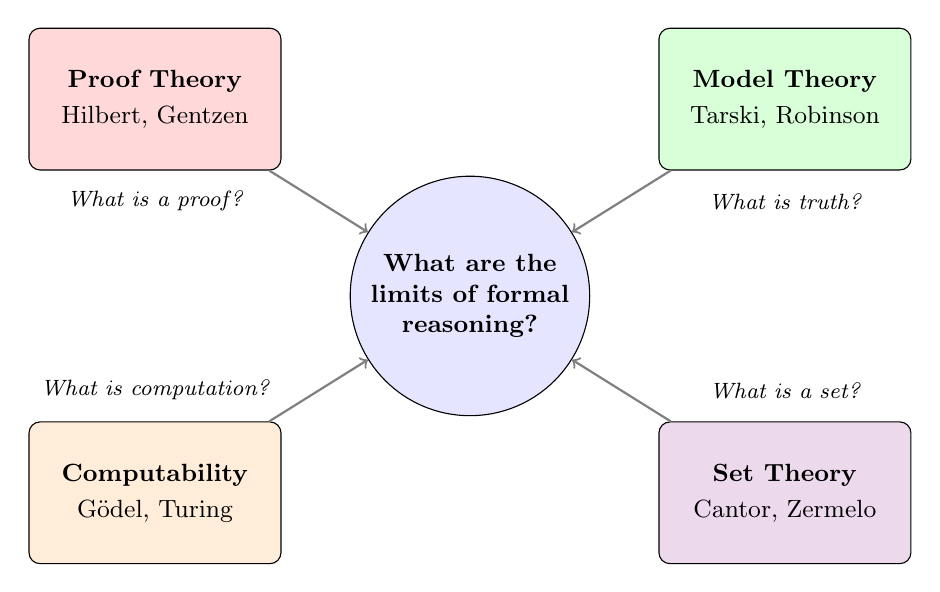
\begin{tikzpicture}[
    pillar/.style={draw, rounded corners, minimum width=3.2cm, minimum height=1.8cm, align=center, font=\small},
    question/.style={font=\footnotesize\itshape, text width=3cm, align=center},
    central/.style={draw, circle, minimum size=2.5cm, align=center, font=\small\bfseries, fill=blue!10},
]
    \node[central] (center) at (0,0) {What are the\\limits of formal\\reasoning?};

    \node[pillar, fill=red!15] (proof) at (-4, 2.5) {\textbf{Proof Theory}\\[2pt]Hilbert, Gentzen};
    \node[pillar, fill=green!15] (model) at (4, 2.5) {\textbf{Model Theory}\\[2pt]Tarski, Robinson};
    \node[pillar, fill=orange!15] (comp) at (-4, -2.5) {\textbf{Computability}\\[2pt]G\"odel, Turing};
    \node[pillar, fill=violet!15] (set) at (4, -2.5) {\textbf{Set Theory}\\[2pt]Cantor, Zermelo};

    \node[question] at (-4, 1.2) {What is a proof?};
    \node[question] at (4, 1.2) {What is truth?};
    \node[question] at (-4, -1.2) {What is computation?};
    \node[question] at (4, -1.2) {What is a set?};

    \draw[->, thick, gray] (proof) -- (center);
    \draw[->, thick, gray] (model) -- (center);
    \draw[->, thick, gray] (comp) -- (center);
    \draw[->, thick, gray] (set) -- (center);
\end{tikzpicture}
\end{center}

\textbf{Proof Theory}: Hilbert's program to formalize mathematics; Gentzen's sequent calculus and cut elimination.

\textbf{Model Theory}: Tarski's semantic definition of truth; studying the relationship between syntax and structures.

\textbf{Computability}: G\"odel's incompleteness; Church-Turing's definition of computability; the halting problem.

\textbf{Set Theory}: Cantor's infinities; ZFC axiomatics; Cohen's independence results.
